\section{Implementation}\label{sec:impl}

The server side, the reference client and all tooling are written in Python; the state transitions are a Lua library that runs inside Redis; the phone apps are native, because detecting new photos needs the operating system's media APIs. Everything described in this chapter is in the submitted source code and was run on the build machine; the Android app was also run on a real phone.

\subsection{Technology Stack}

\begin{table}[H]
\centering
\small\stripes
\begin{tabularx}{\linewidth}{L{2.6cm}L{4.4cm}Y}
\headrow \hd{Layer} & \hd{Technology} & \hd{Why this choice}\\
Edge proxy & Caddy 2 & TLS 1.3 with automatic certificates, HTTP/3 and \texttt{Alt-Svc} built in, reverse proxy with load balancing \\
Services & Python 3.12, FastAPI, uvicorn (uvloop, httptools) & One asynchronous event loop per process handles thousands of open sockets; HTTP and WebSocket in one framework \\
State and events & Redis 7.2, Redis Functions (Lua), Streams & Atomic multi-key transitions in one round trip; a durable, ordered, trimmable event log \\
Accounts & Postgres 16, SQLAlchemy 2 (async), asyncpg, Alembic & Durable, relational, migrations under version control \\
Wire format & Protocol Buffers 5 & Compact binary bodies and WebSocket frames, one schema for Python, Kotlin and Swift \\
Tokens & PyJWT with Ed25519 (EdDSA) & Small, fast signatures; public keys published as a JWKS for rotation \\
Images & Pillow, pillow-heif in a sandboxed subprocess & JPEG, PNG, WebP and HEIC decoding with memory and CPU limits \\
Checksums & \texttt{hashlib} SHA-256, \texttt{google-crc32c} & Hardware-accelerated; 1.8\,GB/s and 11.4\,GB/s on one core \\
Push & firebase-admin (FCM), aioapns (APNs) & Wake-up hints for Android and iOS \\
Android & Kotlin, Jetpack Compose, WorkManager, Room, OkHttp, Cronet & Background work that survives process death; HTTP/3 through Cronet \\
iOS & Swift 6, PhotonKit package, SwiftUI & Shared core library, tested on Linux \\
\end{tabularx}
\caption{Technology stack}\label{tab:stack}
\end{table}

\subsection{File Inventory}

\begin{table}[H]
\centering
\small\stripes
\begin{tabularx}{\linewidth}{L{3.3cm}L{4.1cm}YC{1.0cm}}
\headrow \hd{Directory} & \hd{File} & \hd{Purpose} & \hd{LOC}\\
\ep{orchestrator/lua/} & \texttt{photon.lua} & All 24 state transitions as Redis Functions & 556 \\
\ep{orchestrator/routes/} & \texttt{events.py} & WebSocket, snapshot, catch-up, close codes & 228 \\
 & \texttt{sessions.py}, \texttt{photos.py} & Create, join, leave, kick, end; announce, recall, report & 275 \\
\ep{orchestrator/} & \texttt{svc.py}, \texttt{jobs.py}, \texttt{push.py} & Function calls, sweepers and recount, FCM/APNs & 453 \\
\ep{imageserver/} & \texttt{pipeline.py} & Chunks with CRC32C, assembly, SHA-256, outbox report & 321 \\
 & \texttt{routes.py}, \texttt{access.py} & Upload and download routes, per-request authorisation & 265 \\
 & \texttt{outbox.py}, \texttt{store.py}, \texttt{sweeper.py} & Durable reports, file layout and promotion, local sweeper & 404 \\
\ep{auth/} & \texttt{app.py}, \texttt{providers.py}, \texttt{tokens.py} & OAuth, PKCE, Google ID tokens, GitHub, refresh rotation & 565 \\
\ep{common/} & \texttt{jwtutil.py}, \texttt{config.py}, \dots & JWT, settings, error contract, Redis pools, metrics & 818 \\
\ep{android/} & 65 Kotlin files & Observer, uploader, receiver, UI, tokens & 7{,}172 \\
\ep{ios/} & PhotonKit and app sources & Upload engine, event sync, PKCE, receive pipeline & 7{,}731 \\
\ep{deploy/} & \texttt{docker-compose.yml}, \texttt{Caddyfile}, \dots & Edge, services, Redis with replica and ACLs, Prometheus & 292 \\
\ep{tests/} & unit, integration, e2e, bench & Server tests and benchmarks & 3{,}365 \\
\hline
\multicolumn{3}{r}{\textbf{All source files, including those not listed (plus 4{,}808 lines of app tests)}} & \textbf{24{,}356} \\
\end{tabularx}
\caption{Main source files and their size in lines of code}\label{tab:files}
\end{table}

\subsection{Server Implementation}

\paragraph{One library of Redis Functions.} Every state transition is a function in one Lua library, loaded with \texttt{FUNCTION LOAD} and called with \texttt{FCALL}: \texttt{create\_session}, \texttt{join}, \texttt{leave}, \texttt{kick}, \texttt{end\_session}, \texttt{announce}, \texttt{report\_stored}, \texttt{report\_rejected}, \texttt{recall}, \texttt{expire\_photo}, \texttt{recount}, \texttt{touch\_lease}, and read-only checks such as \texttt{upload\_check}, \texttt{download\_check}, \texttt{snapshot} and \texttt{events\_since}. Redis runs each function to completion before serving any other command, so every check and every write of one transition happen as one atomic step on the server, in one network round trip. Unlike loose \texttt{EVAL} scripts, functions survive a restart and replicate to the replica. Each function declares only keys of one session, which share the \texttt{\{sid\}} hash slot, so the library can later move to Redis Cluster unchanged.

\paragraph{Three services.} Auth, the orchestrator and the image server are separate FastAPI applications with their own Redis ACL user. The orchestrator can run any number of replicas behind the proxy without sticky routing, because a WebSocket reads its events from the Redis stream, not from the process that handled the upload.

\paragraph{Connection pools sized for blocking reads.} Each open WebSocket holds one Redis connection in \texttt{XREAD BLOCK}. These connections come from a separate blocking pool without a socket timeout (200 per replica by default); the pool for ordinary commands has 500 connections, and callers wait up to 5\,s for a free one instead of failing. Both settings came from measurements (Section~\ref{sec:bugs}).

\paragraph{Durability on the image server.} The image server writes each upload's state to disk before it replies, and writes a pending-report record before it reports to the orchestrator. A crash between storing a file and reporting it is recovered at start-up from that record. Files are promoted to their final path \texttt{photos/\{sid\}/\{sha256\}/} only after the orchestrator answers \texttt{200}, with an atomic rename and \texttt{fsync}.

\subsection{Network Edge and Deployment}

Figure~\ref{fig:deploy} shows the deployment on one host with Docker Compose. Only Caddy publishes ports: 443/tcp for HTTPS and WebSocket, 443/udp for QUIC, and 80/tcp for certificate challenges and redirects. Every service and store sits on a private Docker network. Redis requires TLS and has one ACL user per service: the image server, for example, can read \texttt{session:*} and refresh upload leases, and nothing else.

\begin{figure}[H]
\centering
\resizebox{0.88\linewidth}{!}{\fig{deploy}}
\caption{Deployment and network topology}\label{fig:deploy}
\end{figure}

The edge configuration fits on one page. The global \texttt{protocols h1 h2 h3} line enables HTTP/3; Caddy then sends \texttt{Alt-Svc: h3=":443"} on HTTP/2 responses, and clients that can use UDP switch over.

\begin{lstlisting}
{ servers { protocols h1 h2 h3 } }            # HTTP/3 (QUIC) with HTTP/2 fallback
{$PHOTON_PUBLIC_HOST} {
    @private path /internal/* /metrics /readyz
    respond @private 404                        # never reachable from outside
    @auth path /v1/auth/* /v1/devices/* /.well-known/*
    handle @auth { reverse_proxy auth:8082 { lb_policy round_robin } }
    handle { reverse_proxy orchestrator:8080 { lb_policy least_conn
                                                stream_timeout 24h } }   # WebSockets
}
{$PHOTON_IMAGE_HOST} {
    @chunks path /v1/uploads/*/chunks/*
    request_body @chunks { max_size 9MB }       # largest chunk is 8 MiB
    reverse_proxy imageserver:8081 { flush_interval -1 }
}
\end{lstlisting}

The services trust \texttt{X-Forwarded-For} only when the direct peer is a configured proxy, so a client cannot forge its address to escape per-IP rate limits. uvicorn's keep-alive timeout (130\,s) is longer than Caddy's upstream keep-alive (2 minutes), so the proxy never reuses a connection the service has just closed.

\subsection{Authentication and Security}

Figure~\ref{fig:oauth} shows the browser sign-in. The \texttt{state} value is stored in Redis for 10 minutes and read with \texttt{GETDEL}, so it works exactly once; the PKCE verifier proves that the app which started the login is the one finishing it; redirect URIs are matched exactly. On Android, Google sign-in uses the system account picker instead: the app gets a single-use nonce from the server, and the server checks the ID token's issuer, audience, expiry and nonce.

\begin{figure}[H]
\centering
\resizebox{0.82\linewidth}{!}{\fig{oauth}}
\caption{Browser sign-in with OAuth 2.0 Authorization Code and PKCE}\label{fig:oauth}
\end{figure}

\begin{table}[H]
\centering
\small\stripes
\begin{tabularx}{\linewidth}{L{4.6cm}Y}
\headrow \hd{Threat} & \hd{Mitigation}\\
Eavesdropping or tampering on any hop & TLS 1.3 everywhere, including Redis and service-to-service calls; QUIC encrypts its transport headers too \\
Stolen authorization code & PKCE: the code is useless without the verifier, which never leaves the phone \\
Replayed or forged login & Single-use \texttt{state} (\texttt{GETDEL}); single-use nonce for Google ID tokens; exact redirect URIs \\
Stolen refresh token & Rotation on every use; reuse outside the 30\,s grace window revokes the whole family \\
Leaked access token & 15-minute lifetime; WebSocket closed with 4001 at expiry; token sent in the first frame, never in a URL \\
Forged hash to poison dedupe & Server recomputes SHA-256; mismatch is a strike; 3 strikes block uploads \\
Malicious image file (decoder exploit, decompression bomb) & Type allow-list, magic bytes, 25\,MB and 100\,MP limits, decoding in a separate process with memory, CPU and wall-clock limits \\
Leaked event or link & Events carry no URL; every download checks JWT, membership, status and expiry; \texttt{no-store} \\
Abuse as free file hosting & 1\,GB per session, 3 live uploads per user and 20 per session, 20 announces a minute, 30-minute retention \\
\end{tabularx}
\caption{Threats and how PHOTON handles them}\label{tab:threats}
\end{table}

\subsection{Android Client}

The Android app is where the networking meets the limits of a mobile operating system (Figure~\ref{fig:android}). Android stops ordinary background services within minutes, so while a session is active the app runs a foreground service with a visible notification, whose \texttt{ContentObserver} only records new photos in a local Room table and enqueues work. A second path, a WorkManager job triggered by a content URI, fires even when the app's process has been killed. WorkManager owns every slow step: hashing, removing GPS data, announcing, uploading with retries, and resuming after the network returns.

\begin{figure}[H]
\centering
\resizebox{0.9\linewidth}{!}{\fig{android}}
\caption{Android client: capture, upload, receive and echo prevention}\label{fig:android}
\end{figure}

On the receiving side, the app shows the thumbnail as soon as the event arrives, then the preview, and fetches the original on Wi-Fi or while charging if the user chose that. Only the original is saved to the gallery, in a \texttt{Pictures/PHOTON} folder, with its original capture time so it lands in the right place in the timeline. A reconcile scan on every start, restart and boot catches anything the observer missed. The app also restarts its service after an app update (\texttt{MY\_PACKAGE\_REPLACED}) and asks the user to exempt it from battery optimisation.

\subsection{iOS Client}

iOS does not let an app run continuously in the background, so the iOS design states this openly: photos taken while the app is suspended are uploaded on its next launch or return to the foreground, and a silent APNs push may wake it briefly. The shared logic is a Swift package, PhotonKit, with the upload engine, chunk planner, PKCE, token manager, event sync and receive pipeline. It builds and its 90 tests pass on Linux with Swift 6.3; the SwiftUI app target has not been compiled, because that needs Xcode on macOS.

\subsection{Testing}

The tests start a real Redis, an embedded Postgres and all three services on random ports. Time is driven through a shared clock module, so expiry and grace windows are tested without waiting. Table~\ref{tab:tests} lists the suites.

\begin{table}[H]
\centering
\small\stripes
\begin{tabularx}{\linewidth}{L{3.6cm}Y}
\headrow \hd{Suite} & \hd{What it proves}\\
Unit & Error contract, ids, one Redis slot per function call, token verification, the decoder against hostile files, push routing \\
\texttt{test\_auth}, sign-in & Single-use \texttt{state}, PKCE, exact redirect URIs, refresh grace window and reuse revocation, no merging by e-mail, Google nonce, GitHub flow \\
\texttt{test\_upload} & Resumable chunks, idempotent \texttt{complete} in every state, hash mismatch, crash recovery through the outbox \\
\texttt{test\_fencing} & One upload per hash, quota races, stale reports fenced out, Redis-loss recovery, recall, strikes \\
\texttt{test\_model} & Random sequences of every transition against the real Lua functions (hypothesis), checking the quota and event invariants after each step \\
\texttt{test\_events} & 1{,}200 events delivered once and in order across random reconnects; resync; close codes; downloads with \texttt{Range} \\
\texttt{test\_retention} & Exact logical expiry, both sweepers, retried deletes, orphans, Redis loss \\
\hline
\textbf{Result} & \textbf{155 server tests pass} (67\,s); 135 Android unit tests and 90 PhotonKit tests pass; \texttt{ruff} clean; \texttt{mypy --strict} clean \\
\end{tabularx}
\caption{Test suites and what they prove}\label{tab:tests}
\end{table}

\subsection{Performance Evaluation}\label{sec:perf}

\subsubsection{Setup}

The benchmark suite (\texttt{scripts/bench.sh}) ran on one laptop: Intel Core i5-13450HX (16 threads), 15\,GB RAM, Python 3.12.3, Redis 7.2.4. Redis, Postgres, all services and the load generator share the machine and, for the HTTP tests, one Python event loop. The numbers are therefore relative measurements of this build over loopback, not production capacity.

\subsubsection{State Transitions and Primitives}

\begin{table}[H]
\centering
\small\stripes
\begin{tabularx}{\linewidth}{YC{1.5cm}C{1.5cm}C{1.5cm}}
\headrow \hd{Operation} & \hd{p50} & \hd{p95} & \hd{p99}\\
\texttt{announce} (new photo), 1{,}000 calls & 0.08\,ms & 0.17\,ms & 0.26\,ms \\
\texttt{report\_stored} with event append & 0.07\,ms & 0.17\,ms & 0.24\,ms \\
\texttt{download\_check} (every download) & 0.07\,ms & 0.15\,ms & 0.28\,ms \\
\texttt{events\_since} (500 events) & 14.4\,ms & 15.3\,ms & 32.1\,ms \\
\texttt{snapshot} (1{,}000 stored photos) & 10.9\,ms & 14.6\,ms & 18.8\,ms \\
\hline
\multicolumn{4}{l}{Throughput with 64 calls in flight: 14{,}038 \texttt{download\_check}/s. Ed25519: sign 34{,}230/s, verify 9{,}842/s.} \\
\multicolumn{4}{l}{SHA-256: 1{,}831\,MB/s; CRC32C: 11{,}403\,MB/s (one core).} \\
\end{tabularx}
\caption{Latency of Redis functions and cost of tokens and checksums}\label{tab:lua}
\end{table}

A state transition costs under a tenth of a millisecond inside Redis, so the atomic design does not limit throughput; the HTTP layer does.

\subsubsection{Announce over HTTP and Little's Law}

Figure~\ref{fig:chart-announce} shows the announce endpoint (JWT check, protobuf decoding, one Lua call and signing an upload token) under 1, 16 and 64 concurrent clients. Throughput rises from 545 to about 700 requests per second and then stays flat: the single service process is saturated. Beyond saturation, extra clients only wait in the queue. Little's law relates the number of requests in the system $L$, the throughput $\lambda$ and the time each request spends in the system $W$:
\begin{equation}\label{eq:little}
  L = \lambda W \quad\Rightarrow\quad W = \frac{L}{\lambda} = \frac{64}{704\ \text{s}^{-1}} \approx 91\ \text{ms}.
\end{equation}
The measured mean is 75\,ms. The remaining 16\,ms is time each request spends inside the load generator before it is timed, because the generator shares the event loop with the services. At 16 clients the prediction is 23\,ms against 19\,ms measured. The model explains the result: latency grows linearly with concurrency once the server is saturated, so capacity is added with more orchestrator replicas, which need no coordination.

\begin{figure}[H]
\centering
\resizebox{0.92\linewidth}{!}{\fig{chart-announce}}
\caption{Announce over HTTP: throughput saturates at about 700 requests/s; latency follows Little's law}\label{fig:chart-announce}
\end{figure}

\subsubsection{Upload Path}

Figure~\ref{fig:chart-upload} breaks the end-to-end upload time into its three phases for four photo sizes, with 1\,MiB chunks sent three at a time. Over loopback the chunk transfer is small; almost all the time is \texttt{complete}, which assembles the file, hashes it, validates and decodes it in a subprocess, makes the thumbnail, writes the metadata and sends the fenced report. On a phone the chunk phase is bounded by the radio link instead.

\begin{figure}[H]
\centering
\resizebox{0.85\linewidth}{!}{\fig{chart-upload}}
\caption{Where upload time goes, by photo size (median of 3)}\label{fig:chart-upload}
\end{figure}

Decoding dominates: even a tiny JPEG costs about 48\,ms, the price of starting a fresh, resource-limited process for every decode, so that a malicious file can exhaust only its own worker. A 12\,MP JPEG costs 97\,ms to validate and 151\,ms for the thumbnail; a 12\,MP HEIC costs about six times as much.

\subsubsection{Event Fan-out and Throughput}

\begin{table}[H]
\centering
\small\stripes
\begin{tabularx}{\linewidth}{YC{1.5cm}C{1.5cm}C{1.5cm}}
\headrow \hd{Measurement} & \hd{p50} & \hd{p95} & \hd{p99}\\
Event appended $\to$ frame received, 10-member session (200 deliveries) & 2.6\,ms & 4.3\,ms & 4.5\,ms \\
Upload start $\to$ last of 10 members received (20 photos) & 159\,ms & 167\,ms & 168\,ms \\
Event appended $\to$ frame received, 153 sockets in 17 sessions (3{,}060 deliveries) & 28.8\,ms & 31.3\,ms & 35.8\,ms \\
\hline
\multicolumn{4}{l}{8 members uploading at once: 48 photos (45\,MB) in 1.94\,s = 24.8 photos/s, 23.2\,MB/s, all stored.} \\
\multicolumn{4}{l}{Load test, 20 sessions $\times$ 5 members: 300 of 300 photos stored, 1{,}200 of 1{,}200 deliveries.} \\
\end{tabularx}
\caption{Event delivery and upload throughput}\label{tab:fanout}
\end{table}

A photo reaches all ten members of a session about 160\,ms after its upload starts, and the fan-out itself (stream to socket) takes under 5\,ms. With 153 sockets, every one of the 3{,}060 events was delivered.

\subsubsection{Real Device Results}\label{sec:device}

The Android app was tested on a Motorola edge 70 fusion with Android 16, connected to the development server over USB (\texttt{adb reverse}) and over Wi-Fi.

\begin{table}[H]
\centering
\small\stripes
\begin{tabularx}{\linewidth}{YL{4.4cm}}
\headrow \hd{Scenario} & \hd{Result}\\
Photo taken with the camera app, PHOTON in the background & Stored 14\,s after capture \\
Test photo written to the gallery, PHOTON in the background & Stored 2.1\,s after it was written \\
Same, after the app's process was killed & Stored 1.8\,s after (service restarted, trigger fired) \\
App updated during a session & Sync resumed without opening the app \\
\end{tabularx}
\caption{Results on a real phone}\label{tab:device}
\end{table}

The 14\,s for a real camera photo includes the time the camera app takes to finish writing the file and publish it to MediaStore, which PHOTON cannot see until it happens.

\subsection{Problems Found by Measurement}\label{sec:bugs}

Running the system on a phone and under load found faults that the functional tests had not. Each was fixed and is now covered by a test.

\begin{table}[H]
\centering
\small\stripes
\begin{tabularx}{\linewidth}{L{4.0cm}L{4.4cm}Y}
\headrow \hd{Symptom} & \hd{Cause} & \hd{Fix}\\
Idle WebSockets on the phone closed with 1011 every few seconds & The Redis client's default 5\,s socket timeout cut every \texttt{XREAD BLOCK 15000} & Blocking pool without a socket timeout, with TCP keepalive \\
150 sockets connecting at once: 50 closed & redis-py's default pool fails the 101st concurrent command & Blocking pools sized by configuration (500 and 200); callers wait up to 5\,s \\
Phone on Wi-Fi could not reach the server & The app was built for \texttt{127.0.0.1}, which on a phone is the phone itself & Install script builds for the laptop's LAN address (Figure~\ref{fig:devnet}) \\
Photos uploaded only while the app was open & Background service stopped; no trigger after process death & Foreground service plus content-URI trigger plus restart after update \\
\end{tabularx}
\caption{Faults found by the device test and the benchmarks}\label{tab:bugs}
\end{table}

\subsection{Screenshots of the System}

The screenshots below come from a real run of the development stack (\texttt{photon-dev}) with two users of the command-line client, Alice and Bob, on one machine.

\begin{figure}[H]
\centering
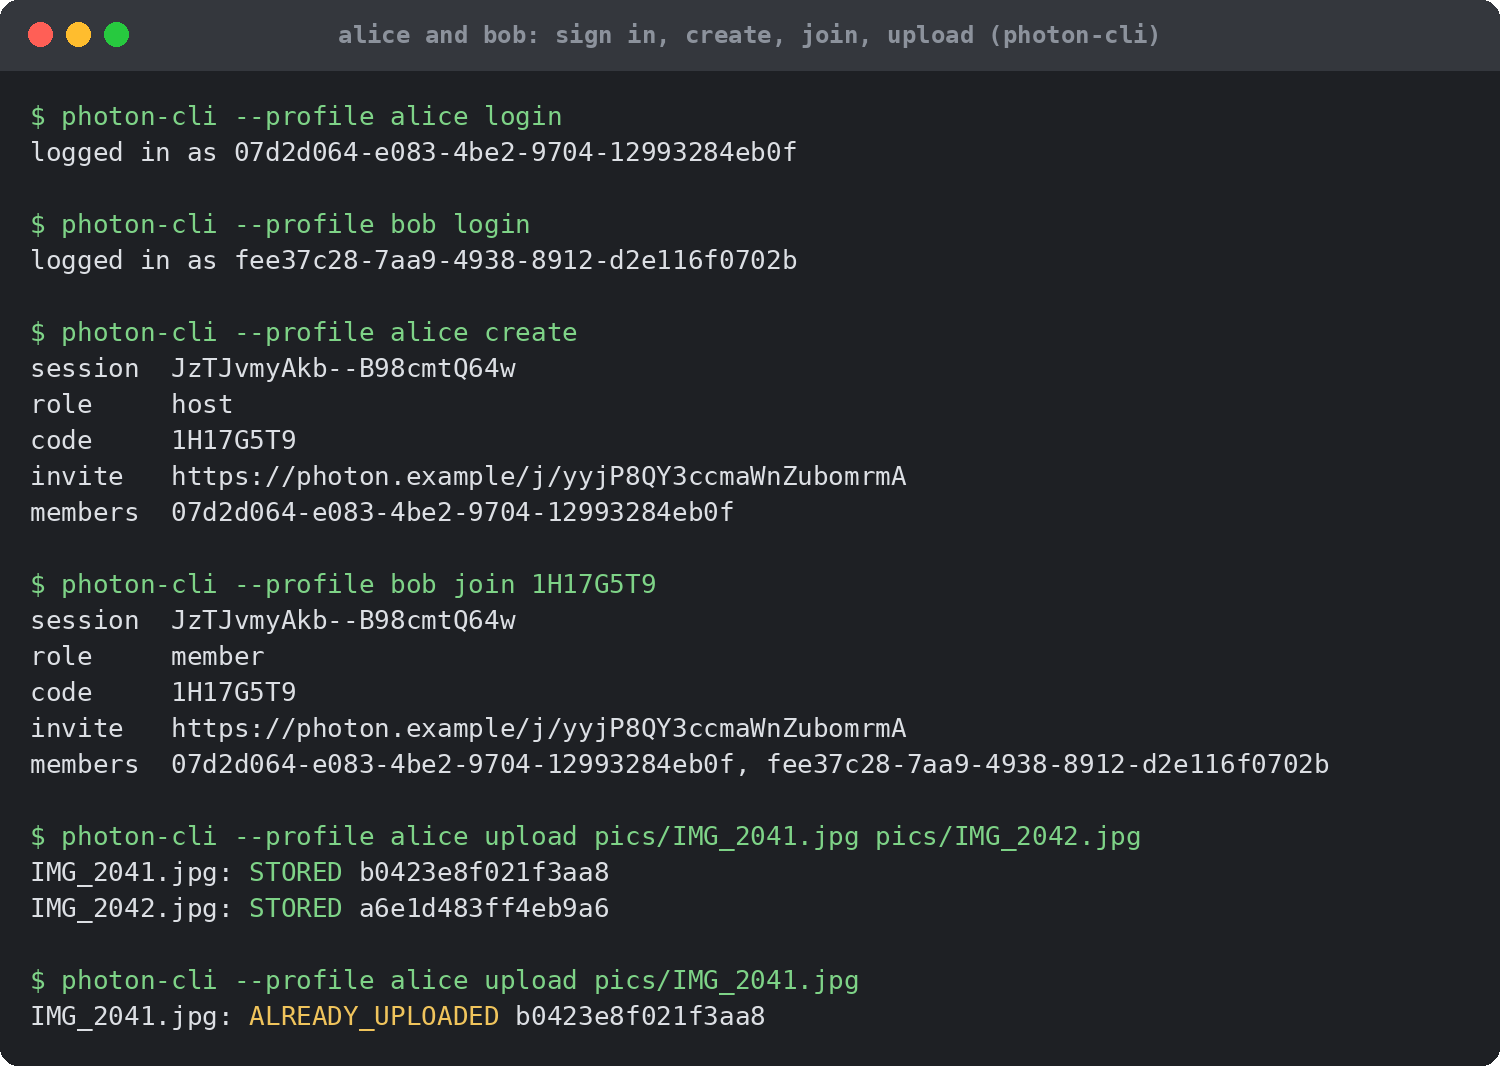
\includegraphics[width=0.78\linewidth]{screens/demo-share.png}
\caption{Alice and Bob sign in, Alice creates a session, Bob joins with the code, Alice uploads two photos, and a repeated upload is answered \texttt{ALREADY\_UPLOADED}}\label{fig:shot-share}
\end{figure}

\begin{figure}[H]
\centering
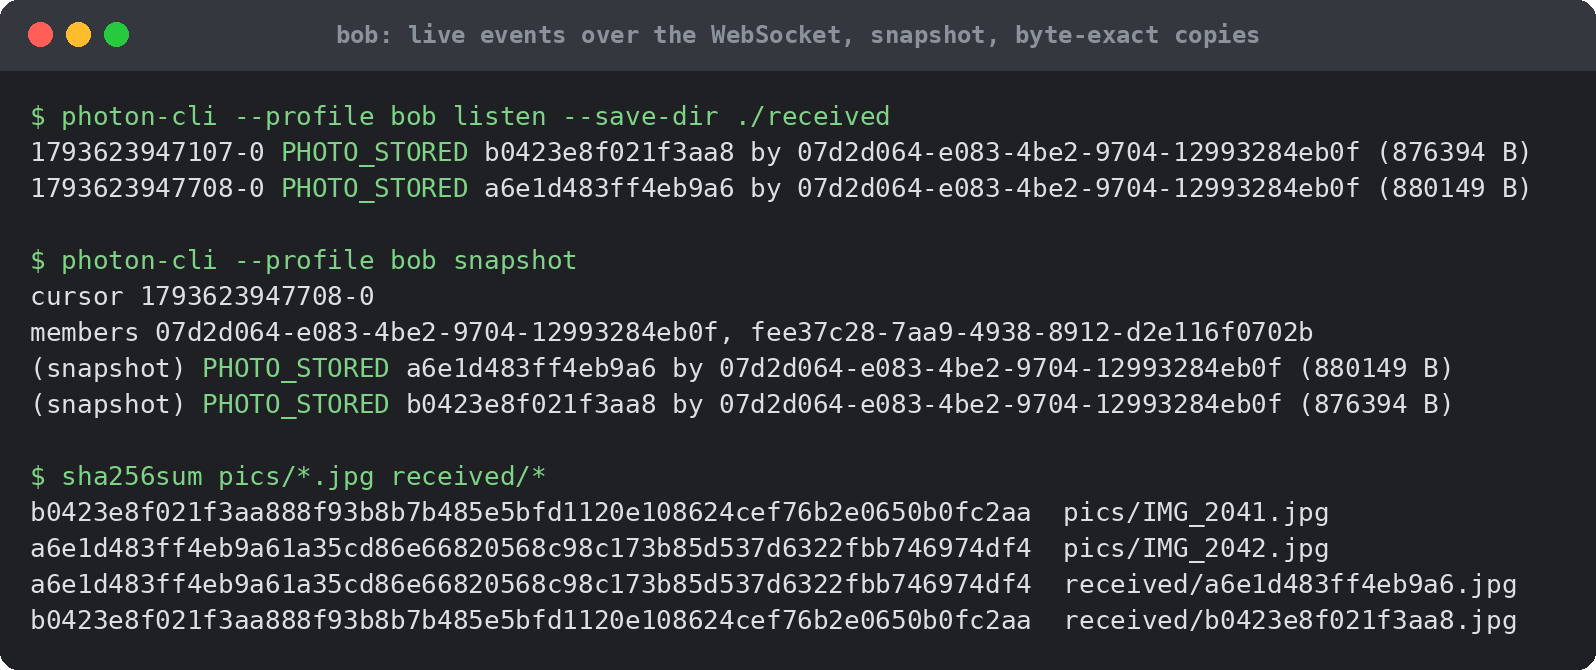
\includegraphics[width=0.86\linewidth]{screens/demo-receive.png}
\caption{Bob receives both \texttt{PHOTO\_STORED} events live over the WebSocket; the snapshot agrees; the received files are byte-identical to the originals (same SHA-256)}\label{fig:shot-receive}
\end{figure}

\begin{figure}[H]
\centering
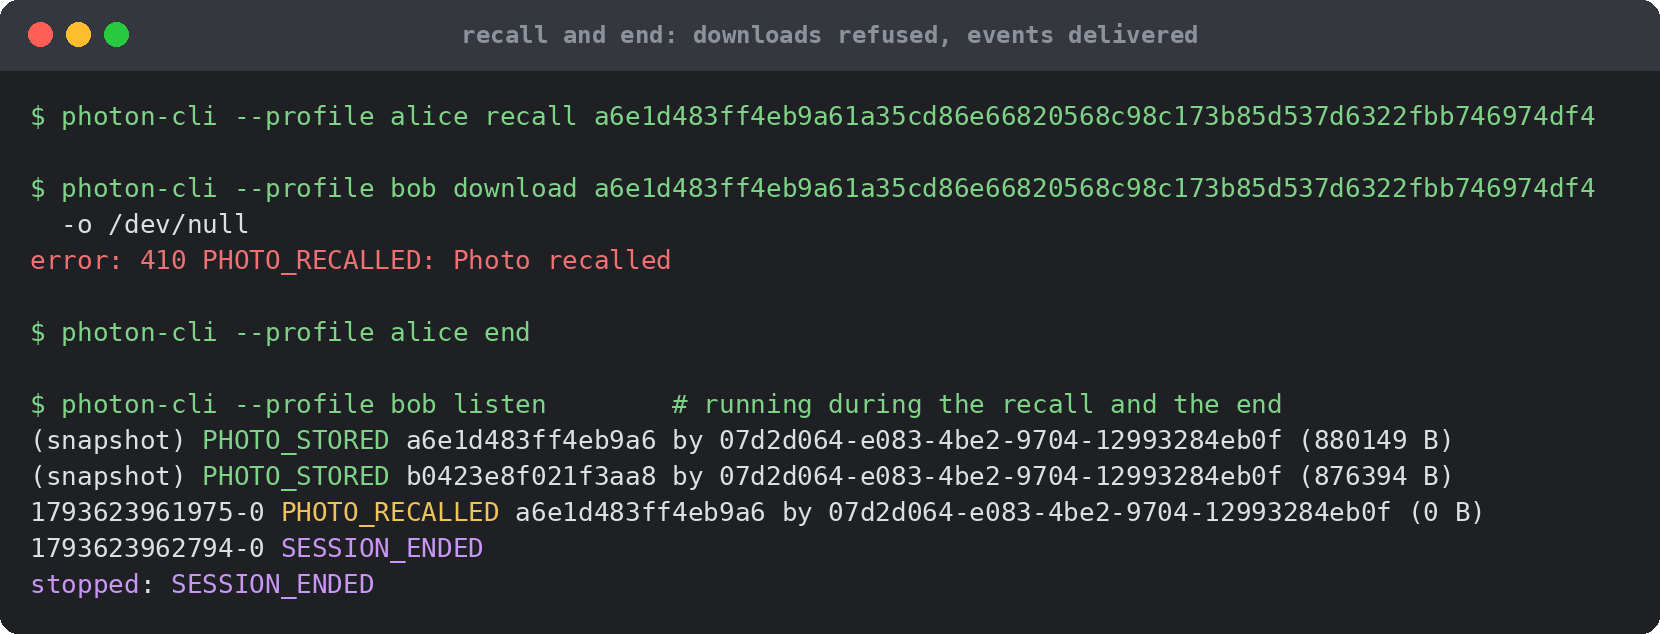
\includegraphics[width=0.86\linewidth]{screens/demo-recall.png}
\caption{Alice recalls a photo: Bob's download is refused with \texttt{410 PHOTO\_RECALLED} and his listener receives \texttt{PHOTO\_RECALLED}, then \texttt{SESSION\_ENDED} when Alice ends the session}\label{fig:shot-recall}
\end{figure}

Figure~\ref{fig:appshots} shows the Android app in a session with two members: developer sign-in, offered because the development server has no Google client configured (a); starting or joining a session (b); the session code, its QR and the members (c); and a photo from the other member, received and saved to the gallery (d).

\begin{figure}[H]
\centering
\begin{tabular}{C{3.45cm}C{3.45cm}C{3.45cm}C{3.45cm}}
\appshot{app-login.jpg}{Sign-in} & \appshot{app-home.jpg}{Start or join} & \appshot{app-session.jpg}{Live session} & \appshot{app-received.jpg}{Photo received}\\[2pt]
\small (a) Sign-in & \small (b) Start or join & \small (c) Live session & \small (d) Photo received \\
\end{tabular}
\caption{The Android app: sign-in, the home screen, a live session with two members, and the same session after a photo from the other member was received and saved}\label{fig:appshots}
\end{figure}

\subsection{Installation Guide}

\subsubsection{Run the Server and the Tests}

The server needs Python 3.12 and a C compiler (Redis 7.2 is built from source); Postgres comes from a Python wheel, so no Docker is needed for development. The Android app needs JDK 17 and the Android SDK.

\begin{pbox}{green}{Quick Start}
\begin{lstlisting}[style=code, backgroundcolor=\color{white}]
scripts/dev-deps.sh                        # builds Redis 7.2 into .devtools/
python3 -m venv .venv && .venv/bin/pip install -e ".[dev]"
.venv/bin/pytest -q                        # 155 tests
.venv/bin/photon-dev                       # API on :8080, image server on :8081
scripts/bench.sh                           # benchmarks -> tests/bench/results/latest.md
\end{lstlisting}
\end{pbox}

\subsubsection{Run on an Android Phone}

A phone reaches the laptop in one of two ways (Figure~\ref{fig:devnet}). Over USB, \texttt{adb reverse} forwards the phone's \texttt{127.0.0.1:8080} through the cable to the laptop, so the app needs no network configuration. Over Wi-Fi, the server listens on all interfaces and the app is built with the laptop's LAN address; both must be on the same subnet.

\begin{figure}[H]
\centering
\resizebox{0.7\linewidth}{!}{\fig{devnet}}
\caption{Two network paths from a test phone to the development server}\label{fig:devnet}
\end{figure}

\begin{pbox}{green}{Phone Setup}
\begin{lstlisting}[style=code, backgroundcolor=\color{white}]
scripts/phone-backend.sh                   # terminal 1: backend reachable from phones
scripts/phone-install.sh                   # terminal 2: USB: adb reverse, build, install, open
scripts/phone-install.sh --lan 10.81.x.y   # or Wi-Fi: build for the laptop's address
scripts/phone-diagnose.sh                  # if photos stop arriving
\end{lstlisting}
\end{pbox}

\subsubsection{Deploy}

\begin{pbox}{green}{Production Deployment}
\begin{lstlisting}[style=code, backgroundcolor=\color{white}]
python3 tools/gen_keys.py deploy/keys          # Ed25519 keys, one per service
scripts/make-certs.sh deploy/certs             # internal CA for Redis TLS
cp deploy/users.acl.example deploy/users.acl   # set Redis passwords
cp deploy/.env.example deploy/.env             # host names, OAuth clients
docker compose -f deploy/docker-compose.yml up -d --build
\end{lstlisting}
\end{pbox}

\subsection{Comparison with Existing Systems}

Table~\ref{tab:compare} compares PHOTON with the tools people use today to exchange event photos. The comparison is based on the publicly documented, default behaviour of each product; ``Partial'' means the feature exists only in a limited form. Figure~\ref{fig:chart-score} totals the table, counting a tick as 1 and Partial as 0.5.

\begin{table}[H]
\centering
\footnotesize\rowcolors{2}{white}{rowalt}
\begin{tabularx}{\linewidth}{YC{1.35cm}C{1.35cm}C{1.35cm}C{1.35cm}C{1.35cm}C{1.35cm}}
\headrow \hd{Feature} & \hd{PHOTON} & \hd{Google Photos} & \hd{iCloud SPL} & \hd{AirDrop} & \hd{Quick Share} & \hd{WhatsApp group}\\
Shares new camera photos with the group automatically & \cm & \pa & \cm & \xm & \xm & \xm \\
Android and iOS members in one group & \cm & \cm & \xm & \xm & \xm & \cm \\
Members need not be near each other & \cm & \cm & \cm & \xm & \xm & \cm \\
No long-lived copy on a server & \cm & \xm & \xm & \cm & \cm & \pa \\
Original quality by default & \cm & \pa & \cm & \cm & \cm & \xm \\
Thumbnail first, original later & \cm & \cm & \cm & \xm & \xm & \cm \\
Uploader can recall a shared photo & \cm & \cm & \cm & \xm & \xm & \cm \\
Time-boxed group joined by code or QR & \cm & \xm & \xm & \xm & \xm & \xm \\
Open source and self-hostable & \cm & \xm & \xm & \xm & \xm & \xm \\
\hline
\rowcolor{boxfill}\textbf{Score / 9} & \textbf{9} & \textbf{5} & \textbf{5} & \textbf{2} & \textbf{2} & \textbf{4.5} \\
\end{tabularx}
\caption{Feature comparison: PHOTON and existing photo-sharing tools}\label{tab:compare}
\end{table}

\begin{figure}[H]
\centering
\resizebox{0.68\linewidth}{!}{\fig{chart-score}}
\caption{Feature score of PHOTON and existing tools (from Table~\ref{tab:compare})}\label{fig:chart-score}
\end{figure}

The table counts only the features PHOTON was designed for. The existing tools are ahead elsewhere: WhatsApp encrypts end to end, while PHOTON's server can read a photo during its 30 minutes; Google Photos and iCloud keep long-term albums and handle video; AirDrop and Quick Share work peer to peer without any server; Apple's own library syncs in the background on iOS; and all of them are tested at a scale far beyond one machine and one phone.
